\section{Some \texorpdfstring{\LaTeX}{LaTeX}~Examples}

\blindtext[1]

\subsection{Tabular}

\begin{tabular}[h]{l|l|l}
  \centering
	Measure & Data & Unit \\ \hline
	1      & 2	  & 3  \\
	4      & 5	  & 6
\end{tabular}

% Example for a Table in BFH-Style with a simple Design
\begin{table}[ht]
   \centering
   \begin{bfhTabular}{lll}
      Stadtteil & Anzahl Personen & Ausländische
      Bevölkerung\\\hline
      Innere Stadt & \num{3748} & \SI{17.9}{\percent}\\\hline
      Länggasse-Felsenau & \num{17976} & \SI{17.1}{\percent}\\\hline
      Mattenhof-Weissenbühl & \num{26895} & \SI{22.4}{\percent}\\\hline
      Kirchenfeld-Schlosshalde & \num{23384} & \SI{13.4}{\percent}\\\hline
      Breitenrain-Lorraine & \num{24082} & \SI{19.4}{\percent}
   \end{bfhTabular}
   \caption{Anzahl Personen, ausländischer Bevölkerungsanteil und Arbeitslosenquote pro
	Stadtteil Ende 2005 (Statistikdienste der Stadt Bern, 2006)}
   \label{tab:tab1}
\end{table}

\begin{table}[ht]
   \centering
   \colorlet{BFH-table}{BFH-MediumBlue!10}
   \colorlet{BFH-tablehead}{BFH-MediumBlue!50}
   \begin{bfhTabular}{lll}
      Stadtteil & Anzahl Personen & Ausländische
      Bevölkerung\\\hline
      Innere Stadt & \num{3748} & \SI{17.9}{\percent}\\\hline
      Länggasse-Felsenau & \num{17976} & \SI{17.1}{\percent}\\\hline
      Mattenhof-Weissenbühl & \num{26895} & \SI{22.4}{\percent}\\\hline
      Kirchenfeld-Schlosshalde & \num{23384} & \SI{13.4}{\percent}\\\hline
      Breitenrain-Lorraine & \num{24082} & \SI{19.4}{\percent}
   \end{bfhTabular}
   \caption{Anzahl Personen, ausländischer Bevölkerungsanteil und Arbeitslosenquote pro
	Stadtteil Ende 2005 (Statistikdienste der Stadt Bern, 2006)}
   \label{tab:tab2}
\end{table}

\begin{table}[ht]
   \centering
   \colorlet{BFH-table}{BFH-MediumRed!10}
   \colorlet{BFH-tablehead}{BFH-MediumRed!50}
   \begin{bfhTabular}{lll}
      Stadtteil & Anzahl Personen & Ausländische
      Bevölkerung\\\hline
      Innere Stadt & \num{3748} & \SI{17.9}{\percent}\\\hline
      Länggasse-Felsenau & \num{17976} & \SI{17.1}{\percent}\\\hline
      Mattenhof-Weissenbühl & \num{26895} & \SI{22.4}{\percent}\\\hline
      Kirchenfeld-Schlosshalde & \num{23384} & \SI{13.4}{\percent}\\\hline
      Breitenrain-Lorraine & \num{24082} & \SI{19.4}{\percent}
   \end{bfhTabular}
   \caption{Anzahl Personen, ausländischer Bevölkerungsanteil und Arbeitslosenquote pro
	Stadtteil Ende 2005 (Statistikdienste der Stadt Bern, 2006)}
   \label{tab:tab3}
\end{table}


\begin{description}
\item[More about Tables] Further information about tables : \url{https://www.latex-tutorial.com/tutorials/tables/}
\item[Long Tables] Further information about long tables : \url{https://www.overleaf.com/learn/latex/tables}
\end{description}


\begin{longtable}{|l|l|l|}
\caption{A sample long table} \label{tab:long} \\


\hline \multicolumn{1}{|c|}{\textbf{First column}} & \multicolumn{1}{c|}{\textbf{Second column}} & \multicolumn{1}{c|}{\textbf{Third column}} \\ \hline 
\endfirsthead

\multicolumn{3}{c}%
{{\tablename\ \thetable{}: \hfill $...$~continued from previous page}} \\
\hline \multicolumn{1}{|c|}{\textbf{First column}} & \multicolumn{1}{c|}{\textbf{Second column}} & \multicolumn{1}{c|}{\textbf{Third column}} \\ \hline 
\endhead

\hline \multicolumn{3}{|r|}{{Continued on next page$...$}} \\ \hline
\endfoot

\hline \hline
\endlastfoot
\centering

One & abcdef ghjijklmn & 123.456778 \\
One & abcdef ghjijklmn & 123.456778 \\
One & abcdef ghjijklmn & 123.456778 \\
One & abcdef ghjijklmn & 123.456778 \\
One & abcdef ghjijklmn & 123.456778 \\
One & abcdef ghjijklmn & 123.456778 \\
One & abcdef ghjijklmn & 123.456778 \\
One & abcdef ghjijklmn & 123.456778 \\
One & abcdef ghjijklmn & 123.456778 \\
One & abcdef ghjijklmn & 123.456778 \\
One & abcdef ghjijklmn & 123.456778 \\
One & abcdef ghjijklmn & 123.456778 \\
One & abcdef ghjijklmn & 123.456778 \\
One & abcdef ghjijklmn & 123.456778 \\
One & abcdef ghjijklmn & 123.456778 \\
One & abcdef ghjijklmn & 123.456778 \\
One & abcdef ghjijklmn & 123.456778 \\
One & abcdef ghjijklmn & 123.456778 \\
One & abcdef ghjijklmn & 123.456778 \\
One & abcdef ghjijklmn & 123.456778 \\
One & abcdef ghjijklmn & 123.456778 \\
One & abcdef ghjijklmn & 123.456778 \\
One & abcdef ghjijklmn & 123.456778 \\
One & abcdef ghjijklmn & 123.456778 \\
One & abcdef ghjijklmn & 123.456778 \\
One & abcdef ghjijklmn & 123.456778 \\
One & abcdef ghjijklmn & 123.456778 \\
One & abcdef ghjijklmn & 123.456778 \\
One & abcdef ghjijklmn & 123.456778 \\
One & abcdef ghjijklmn & 123.456778 \\
One & abcdef ghjijklmn & 123.456778 \\
One & abcdef ghjijklmn & 123.456778 \\
One & abcdef ghjijklmn & 123.456778 \\
One & abcdef ghjijklmn & 123.456778 \\
One & abcdef ghjijklmn & 123.456778 \\
One & abcdef ghjijklmn & 123.456778 \\
One & abcdef ghjijklmn & 123.456778 \\
One & abcdef ghjijklmn & 123.456778 \\
One & abcdef ghjijklmn & 123.456778 \\
One & abcdef ghjijklmn & 123.456778 \\
One & abcdef ghjijklmn & 123.456778 \\
One & abcdef ghjijklmn & 123.456778 \\
One & abcdef ghjijklmn & 123.456778 \\
One & abcdef ghjijklmn & 123.456778 \\
One & abcdef ghjijklmn & 123.456778 \\
One & abcdef ghjijklmn & 123.456778 \\
One & abcdef ghjijklmn & 123.456778 \\
One & abcdef ghjijklmn & 123.456778 \\
One & abcdef ghjijklmn & 123.456778 \\
One & abcdef ghjijklmn & 123.456778 \\
One & abcdef ghjijklmn & 123.456778 \\
One & abcdef ghjijklmn & 123.456778 \\
One & abcdef ghjijklmn & 123.456778 \\
One & abcdef ghjijklmn & 123.456778 \\
One & abcdef ghjijklmn & 123.456778 \\
One & abcdef ghjijklmn & 123.456778 \\
One & abcdef ghjijklmn & 123.456778 \\
One & abcdef ghjijklmn & 123.456778 \\
One & abcdef ghjijklmn & 123.456778 \\
One & abcdef ghjijklmn & 123.456778 \\
One & abcdef ghjijklmn & 123.456778 \\
One & abcdef ghjijklmn & 123.456778 \\
One & abcdef ghjijklmn & 123.456778 \\
One & abcdef ghjijklmn & 123.456778 \\
One & abcdef ghjijklmn & 123.456778 \\
One & abcdef ghjijklmn & 123.456778 \\
One & abcdef ghjijklmn & 123.456778 \\
One & abcdef ghjijklmn & 123.456778 \\
One & abcdef ghjijklmn & 123.456778 \\
One & abcdef ghjijklmn & 123.456778 \\
One & abcdef ghjijklmn & 123.456778 \\
One & abcdef ghjijklmn & 123.456778 \\
One & abcdef ghjijklmn & 123.456778 \\
One & abcdef ghjijklmn & 123.456778 \\
One & abcdef ghjijklmn & 123.456778 \\
\end{longtable}
 

\subsection{Math}
%% Mathematical equations
\begin{align}
\left(\begin{array}{r}
\dot{x_{1}} \\                                              
\dot{x_{2}} \\ 
\dot{x_{3}} \\                                 
\end{array}\right) =
\left[\begin{array}{rrr}
0 & 1 & 0 \\                                              
0 & -\frac{b_{f}}{J} & \frac{K_{m}}{J} \\
0 & -\frac{K_{g}}{L} & \frac{R}{L} \\                                      
\end{array}\right]
\left(\begin{array}{r}
x_{1} \\                                              
x_{2} \\ 
x_{3} \\                                 
\end{array}\right) +
\left[\begin{array}{rr}
0 & 0 \\                                              
-\frac{1}{J} & 0 \\ 
0 & \frac{1}{L} \\                                 
\end{array}\right]
\left(\begin{array}{r}
t_{L} \\                                              
v_{a} \\                                 
\end{array}\right)
\end{align}

\subsection{Include pictures}

\begin{figure}[H]
  \centering
  
\includegraphics[width=.8\textwidth]{placeholder}
  \caption{Some meaningful caption}
  \label{fig:placeholder:1}
\end{figure}


\begin{figure}[h!]
  \centering
  \begin{minipage}{.4\textwidth}
  	\centering
	
\includegraphics[width=\textwidth]{placeholder}
	\caption{PLACEHOLDER}
	\label{fig:placeholder:2}
  \end{minipage}
  \hspace{1em}
  \begin{minipage}{.4\textwidth}
	\centering
	
\includegraphics[width=\textwidth]{placeholder}
	\caption{PLACEHOLDER}
	\label{fig:placeholder:3}
  \end{minipage}%
\end{figure}


%% Source code is stored in the listings folder and will be included from there using its relative path.
\subsection{Code Example}

{
  \thicklines
% \thinlines
\lstinputlisting[style=bfh-c,language=C,caption={My very first C program.},label={lst:hello}]{listings/expl_hello.c}
}
I developed this very nice application writing "Hello World" to my terminal.
The implementation is shown in listing~\ref{lst:hello}.


%% Examples holding dummy content
\subsection{Draw boxes}
\begin{bfhBox}[BFH-DarkPurple]{Purple}
	Note\\
\end{bfhBox}

\blindtext[1]

\begin{bfhBox}[BFH-MediumBlue]{Blue}
	Note\\
\end{bfhBox}

\blindtext[1]

\begin{bfhBox}[BFH-DarkRed]{Red}
	Note\\
\end{bfhBox}

\blindtext[2]

\begin{bfhAlertBox}
  An alert box.
\end{bfhAlertBox}

\begin{bfhWarnBox}
  A warning box.
\end{bfhWarnBox}

\begin{bfhNoteBox}
  A note box.
\end{bfhNoteBox}

\begin{bfhRecycleBox}
  A recycle box.
\end{bfhRecycleBox}


\begin{bfhBox}{No color set}
	Some BFH box without color option set. Using default.\\
\end{bfhBox}


\blindtext[3]


\subsection{Some Item-list}
Sometimes you explain this and that using a bullet points.
This can be done in \LaTeX\ using an item list in a item environment.

\begin{itemize}
\item My first item
\item The second
\item $\cdots$
\item $\cdots$
\end{itemize}

It is also possible to nest such environment and/or enumerate.
\begin{itemize}
\item My first item
\begin{enumerate}
\item My first enumerated item
\item The second
\item $\cdots$
\end{enumerate}
\item The second
\begin{enumerate}
\item An other enumerated item
\item $\cdots$
\item $\cdots$
\end{enumerate}
\end{itemize}


\subsection{Multi column environment}
Split a part of a document in multiple columns is not so easy with WYSIWYG tools.
Whit multicols \LaTeX\ package$\cdots$ well you may know.

\begin{multicols}{3}
\begin{itemize}
\item My first item
\item The second
\item $\cdots$
\item $\cdots$
\end{itemize}
\begin{itemize}
\item My first item
\item The second
\item $\cdots$
\item $\cdots$
\end{itemize}
\begin{itemize}
\item My first item
\item The second
\item $\cdots$
\item $\cdots$
\end{itemize}
\end{multicols}


\blindtext[1]

\begin{multicols}{2}
  \blindtext[1]
\end{multicols}

\begin{multicols}{3}
  \blindtext[1]
\end{multicols}

\begin{multicols}{2}
  \blindtext[1]
\end{multicols}


\begin{multicols}{3}
\begin{itemize}
\item My first item
\item The second
\item $\cdots$
\item $\cdots$
\end{itemize}
\blindtext[1]
\columnbreak
\begin{itemize}
\item My first item
\item The second
\item $\cdots$
\item $\cdots$
\end{itemize}
\end{multicols}

%% forced page break
\newpage

\subsection{Use Figures}

\begin{figure}[h!]
  \centering
  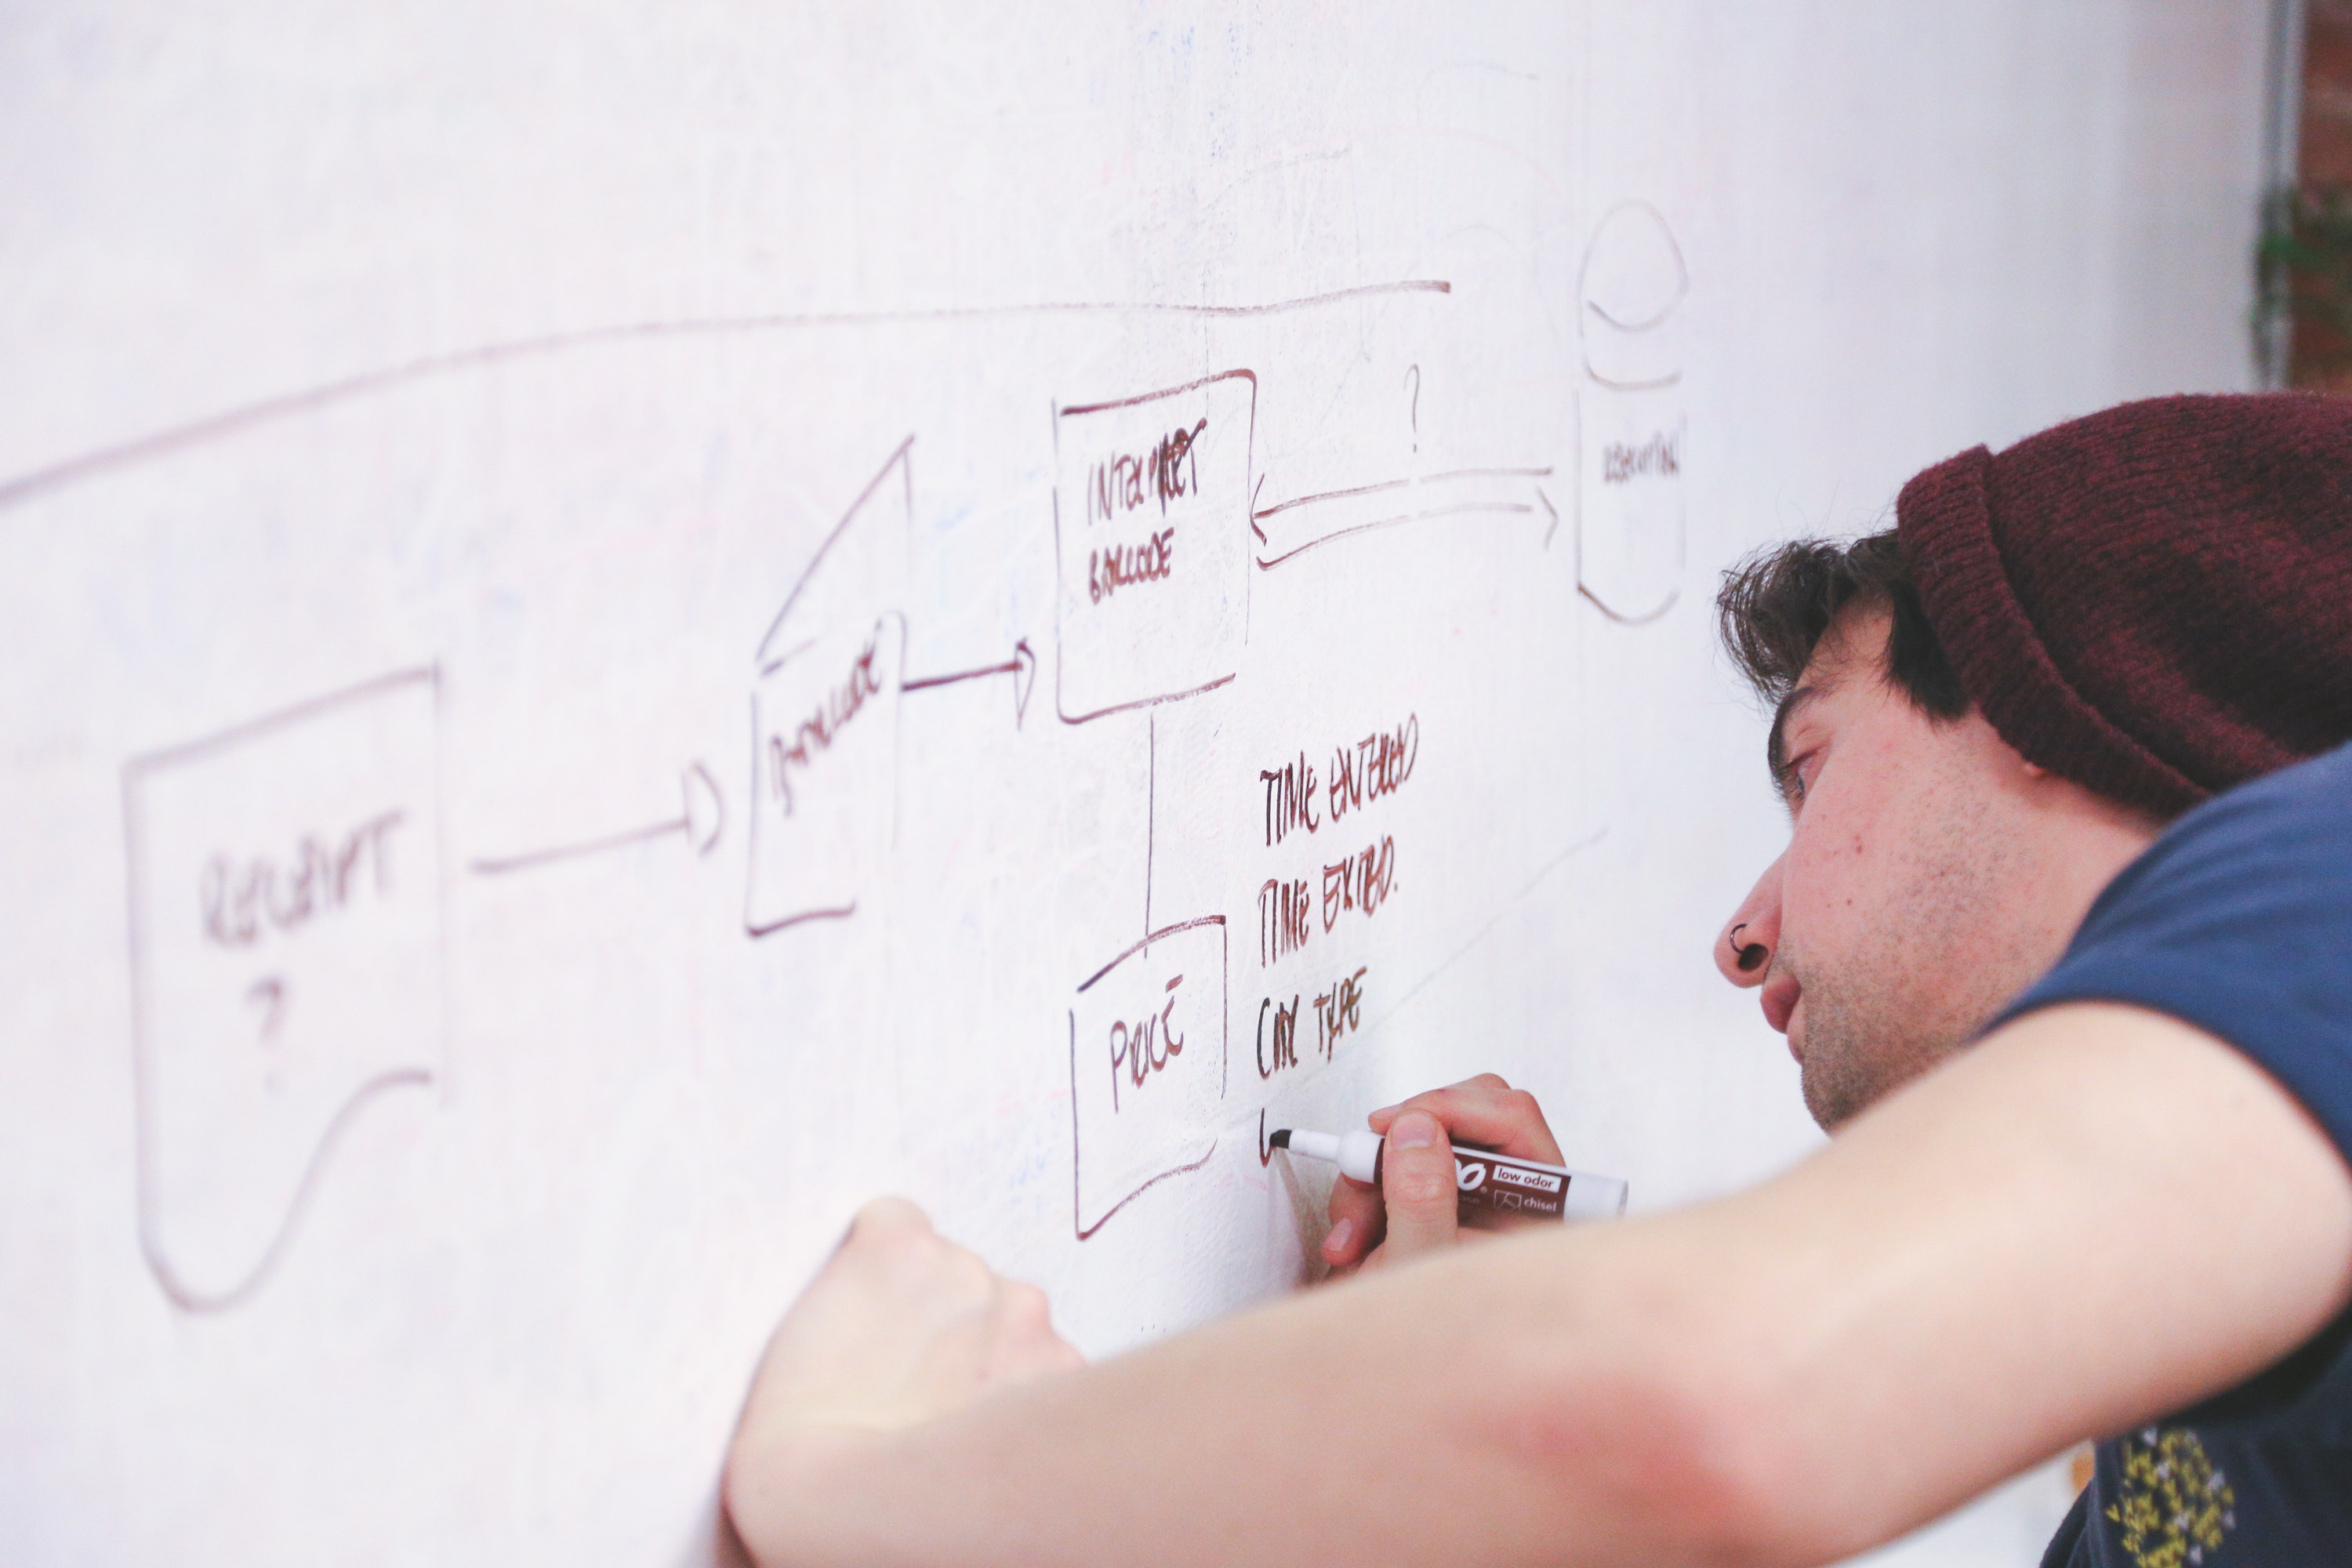
\includegraphics[width=.8\textwidth]{bg-masthead}
  \caption{An example of including a PDF figure.}
  \label{fig:expl_master}
\end{figure}

\begin{figure}[h!]
  \centering
  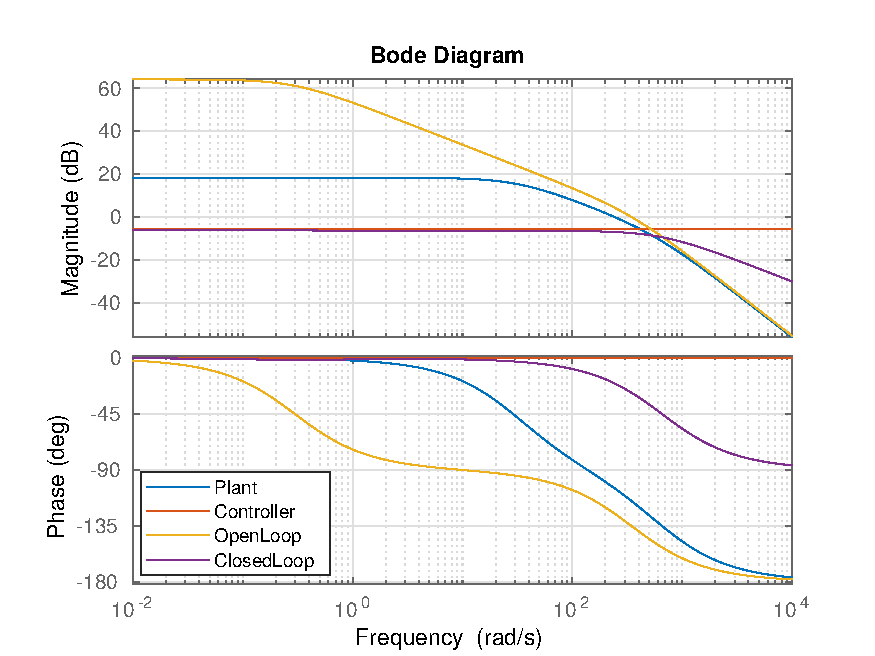
\includegraphics[width=.8\textwidth]{expl_bode}
  \caption{An example of including a PDF figure.}
  \label{fig:expl_bode}
\end{figure}
\clearpage

\subsubsection{Use Subfigures}
These subfigures requires the package \texttt{subcaption}.

\begin{figure}[h!]
     \centering
     \begin{subfigure}[b]{0.3\textwidth}
         \centering
         
\includegraphics[width=\textwidth]{placeholder}
         \caption{$y=x$}
         \label{fig:y equals x}
     \end{subfigure}
     \hfill
     \begin{subfigure}[b]{0.3\textwidth}
         \centering
         
\includegraphics[width=\textwidth]{placeholder}
         \caption{$y=3sinx$}
         \label{fig:three sin x}
     \end{subfigure}
     \hfill
     \begin{subfigure}[b]{0.3\textwidth}
         \centering
         
\includegraphics[width=\textwidth]{placeholder}
         \caption{$y=5/x$}
         \label{fig:five over x}
     \end{subfigure}
        \caption{Three simple graphs}
        \label{fig:three graphs}
\end{figure}


\section{Example Text With Indices}
In this example, several keywords\index{keywords} will be used 
which are important and deserve to appear in the Index\index{Index}.

Terms like generate\index{generate} and some\index{others} will 
also show up.

\section{Example Text With Glossary}
This \Gls{zynq} introduction summary has been written for bachelor students due to the introduction workshop in the ``Embedded Systems'' course at Bern University of Applied Sciences. The topic \Gls{soc} is introduced by using Xilinx' \Gls{apsoc} platform \Gls{zynq}. The subsequent summery is a brief introduction only. It is based on several tutorials in the field of \Gls{soc} such as the \Gls{zbook} or Xilinx' \Gls{apsoc} manual. We think the script provides a good introduction and helps getting the overall picture of the \Gls{soc} basics. In addition we reference to our wiki tutorials that provide lots of information on how to get started with the \Gls{zboard}.\\

Hey folks let's do an \Gls{asic} design and develop some awesome \Gls{rtos}! Yea \Gls{arm} is nice but we can do better, can we?

\section{Example Text With Citations}
%% Text with citations

This document is an example of \Gls{BibTeX} using in bibliography management. Three items 
are cited: The \LaTeX\ Companion book \cite{latexcompanion}, the Einstein
journal paper \cite{einstein}, and the Donald Knuth's website \cite{knuthwebsite}. 
The \LaTeX\ related items are \cite{latexcompanion,knuthwebsite}.

